%!TEX root = ../diplom.tex

\section{Моделирование процесса измерения}

Важным преимуществом орбитального радиовысотомера по сравнению с другими
радиолокаторами является то, что теоретические модели рассеяния хорошо
описывают свойства радиолокационного сигнала, отраженного морской поверхностью.
В результате алгоритмы обработки получены не с помощью регрессионного анализа,
а основаны на аналитических формулах для формы отраженного импульса.

Если, например, говорить об определении скорости ветра по сечению обратного
рассеяния для скаттерометра, то алгоритмы были получены благодаря применению
регрессионного анализа массива данных, сформированного из контактных измерений
скорости и направления ветра (морские буи) и сечения обратного рассеяния,
измеренного радиолокатором. Погрешность оценки (не измерения!) скорости ветра
по сечению обратного рассеяния обусловлена неоднозначностью связи скорости
ветра и сечения обратного рассеяния.

У радиовысотомера при определении с высоты значительного волнения происходит
именно процесс измерения, т.к. существует однозначная связь формы переднего
фронта отраженного импульса и высоты значительного волнения, которая выражается
через известную формулу. В данном точность измерения ограничивается параметрами
радиолокатора, в частности, длительностью излучаемого импульса и частотой
дискретизации.

При измерении расстояния от радиолокатора до среднего уровня морской
поверхности алгоритм также опирается аналитические формулы и модели, например,
учитывает особенности распространения электромагнитного излучения в атмосфере и
ионосфере, что позволяет обеспечить высокую точность.

Благодаря возможности достоверного теоретического  описания рассеяния
электромагнитного излучения взволнованной водной поверхностью, численное
моделирование является эффективным инструментом для моделирования работы
радиовысотомера и отладки алгоритмов обработки. С его помощью можно провести
численный эксперимент и рассмотреть по отдельности и в комплексе влияние
множества факторов, которые влияют на точность измерений.

\subsection{Схема измерения}%
\label{sub:skhema_izmereniia}

Преимущество численного моделирования по сравнению с экспериментом состоит в
том, что достаточно просто провести сравнение различных схем измерения и
оценить их эффективность для решения конкретной задачи. Однако для этого
необходимо подробно описать и перевести в числовую форму все важные для
моделирования параметры схемы измерения. В результате это позволит провести
полноценный <<численный>> эксперимент.  Для описания схемы измерения необходимо
задать угол зондирования (падения) $\theta_0$, высоту орбиты $H_0$, скорость и
направление движения $v_{rad}$, и направление зондирования $\phi_{rad}$. На рис.\ref{fig:geometry} показана схема измерения. 

Расстояние от радиолокатора до точки отражения на плоскости $XY$ равно $R_0$ .
Для определенности выберем направление движения радиовысотомера вдоль оси $X$.


Для плоской поверхности формирование отраженного импульса начинается при
касании поверхности передним фронтом падающего импульса в точке непосредственно
под радиовысотомером. Это кратчайшее расстояние от радиовысотомера до
поверхности. На рис.\ref{fig:wave_form} показан пример изменения формы
рассеивающей площадки и формы отраженного импульса в зависимости от времени.

\begin{figure}[h]
    \centering
    \hfill
    \begin{subfigure}{0.25\linewidth}
        \centering
        \includesvg{wave_front2}
    \end{subfigure}
    \hfill
    \begin{subfigure}{0.25\linewidth}
        \centering
        \includesvg{wave_front3}
    \end{subfigure}
    \hfill
    \begin{subfigure}{0.25\linewidth}
        \centering
        \includesvg{wave_front4}
    \end{subfigure}
    \label{fig:wave_form}
    \caption{Геометрическая интерпретация формы отраженного импульса}
\end{figure}
\subsection{Влияние морского волнения на форму отраженного импульса}%
\label{sub:vliianie_morskogo_volneniia_na_vormu_otrazhennogo_impul_sa}


При малых углах падения механизм обратного  рассеяния является квазизеркальным
и отражение происходит на участках волнового профиля, ориентированных
перпендикулярно падающему излучению. Тогда в формировании отраженного сигнала
будут участвовать только площадки, ориентированные нормально к излучению. 
Поэтому для моделирования рассеяния нам необходимо знать не только высоту в
точке, но и уравнение касательной к ней плоскости, для этого необходимо знать
наклоны $\zeta_x$ и  $\zeta_y$ в искомой точке
\footnote{Под словосочетанием <<отражающая точка>>, конечно, подразумевается
    физически малая площадка с большим радиусом кривизны, характерные размеры  которой больше длины волны
радиолокатора}. 

Зная координаты радиолокатора  $(x_{rad},y_{rad},H_0)$, координаты точки на
поверхности $(x,y,\zeta)$, можем из геометрии (см. рис. \ref{fig:local_theta})

\begin{equation}
    \label{eq:local_theta}
    \cos \theta = \frac
    {\zeta_x (x - x_{rad}) + \zeta_y (y - y_{rad}) - (\zeta - H_0) }
        {
           \sqrt{(x - x_{rad})^2 + (y - y_{rad})^2 + (\zeta - H_0)^2 }
           \sqrt{\zeta_x^2 + \zeta_y^2 + 1}
        }
\end{equation}

Вероятность того, что угол $\theta$ будет точно равен нулю и произойдет
зеркальное отражение для случайной выбранной точки очень мала, поэтому имеет
смысл рассматривать квазизеркальное отражение и вводить ограничение на
максимально допустимый локальный угол отражения. 

Нахождение всех зеркальных точек на характерном пятне радиолокатора  $> 1
\text{ км}^2$ представляет собой ресурсоемкую задачу. Но поскольку формирование
импульса носит статистический характер, то мы может выбирать гораздо меньшую
выборку зеркальных точек. 

Процесс создания такой выборки продемонстрирован на рис. \ref{fig:mirror:a}-\ref{fig:mirror:c}. 

Для смоделированной поверхности  рис. \ref{fig:mirror:a} для некоторой
выборки точек вычисляются по формуле \eqref{eq:local_theta} локальные углы
падения. Квазизеркальными позже считаются те, для которых угол меньше одного
градуса $\theta < 1^\circ$. Выборку можно делать несколькими способами,
например создать её выбирая случайные точки на координатной сетке или проходить
координатную сетку с равномерным шагом. 
Выборка на рис. \ref{fig:mirror:b} и \ref{fig:mirror:c} получена вторым
способом. 

\begin{figure}[h!]
    \centering
    \def\svgwidth{0.75\linewidth}
    \includesvg{local_theta}
    \caption{Геометрия определения локального угла падения. Красной линией
    обозначена касательная плоскость к рассматриваемой отражающей точке
$(x,y,\zeta)$}
    \label{fig:local_theta}
\end{figure}

\begin{figure}[h]
    \centering
    \begin{subfigure}{0.65\linewidth}
        \centering
        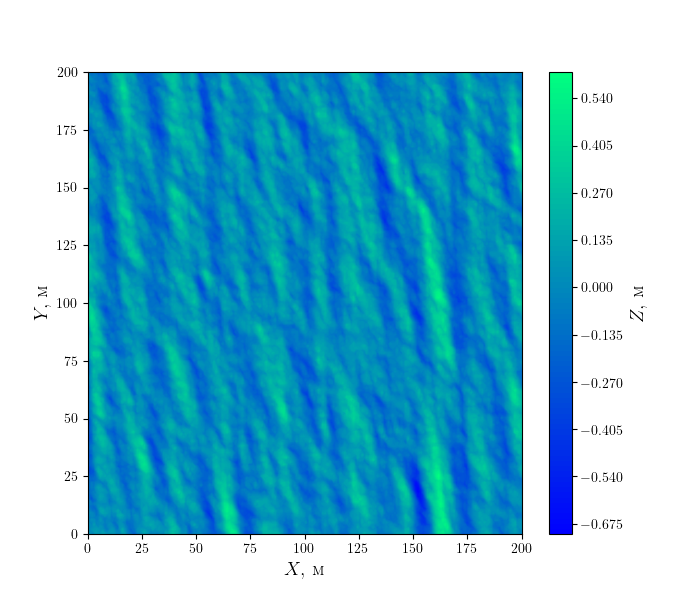
\includegraphics[width=\linewidth]{fig/impulse/fig1}
        \caption{Моделирование поверхности при скорости ветра $U=5$ м/с}
        \label{fig:mirror:a}
    \end{subfigure}
    \begin{subfigure}{.49\linewidth}
        \centering
        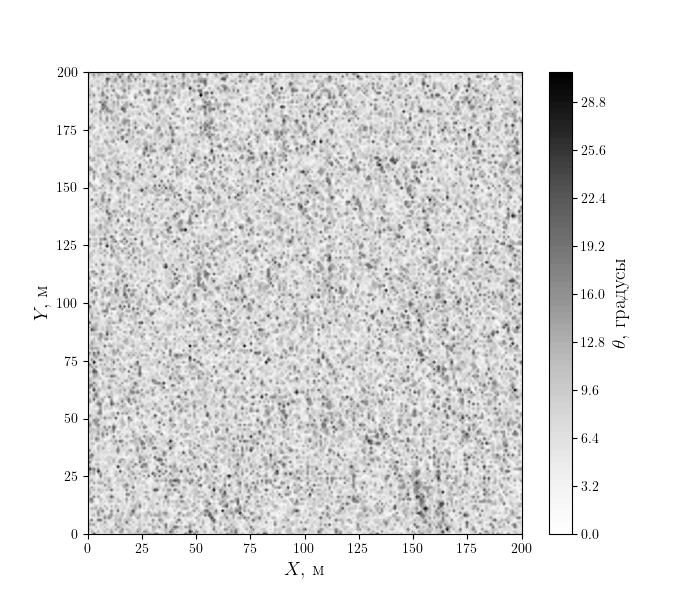
\includegraphics[width=\linewidth]{fig/impulse/fig2}
        \caption{Локальный угол отражения от поверхности для радиолокатора
        находящегося на высоте $H=1000$ км в точке с координатой (100, 100)}
        \label{fig:mirror:b}
    \end{subfigure}
    \begin{subfigure}{.49\linewidth}
        \centering
        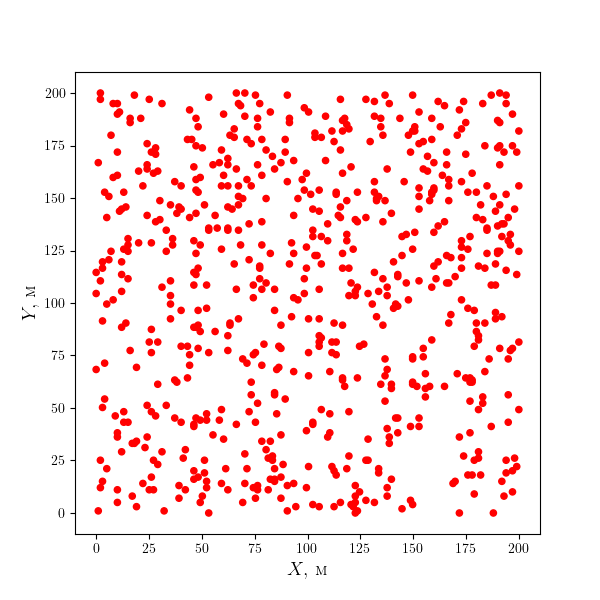
\includegraphics[width=\linewidth]{fig/impulse/fig3}
        \caption{Положение зеркальных точек поверхности \ref{fig:mirror:a} для
        радиолокатора находящегося над точкой (100,100) }
        \label{fig:mirror:c}
    \end{subfigure}
    \label{fig:mirror}
    \caption{}
\end{figure}

Теперь, для вычисления поля вблизи приемной антенны радиолокатора нам
необходимо просуммировать отраженное от квазизеркальных точек поле
(см.рис. \ref{fig:mirror:c}).  


Как было сказано с предыдущих разделах, амплитуда поля излученного антенной
спадает по гиперболическому закону. Тогда амплитуда поля вблизи точки отражения
$(x,y,\zeta)$
будет определяться как (см. геометрию задачи на рис. \ref{fig:local_theta})
\begin{equation}
    \label{eq:}
    E_{sur} \sim \frac{E_0}{R_1} e^{-ikR_1} \cdot G(x,y,\theta_0), 
\end{equation}
Следовательно, вблизи приемной антенны амплитуду можно записать как
\begin{equation}
    \label{eq:E}
    E \sim \frac{E_{sur}}{R_1} e^{-ikR_1} \cdot G(x,y,\theta_0) =
    \frac{E_0}{R_1^2} e^{-2ikR_1} \cdot G^2(x,y,\theta_0), 
\end{equation}

Остается только проинтегрировать уравнение \eqref{eq:E} по всем отражающим
точкам 
\begin{equation}
    \label{eq:}
    E \sim \sum\limits_{i=1}^{M} \frac{E_0}{R_i^2} \exp{-2ikR_i}
    G^2(x,y,\theta_0)
\end{equation}
где $M$ -- количество точек,  $x_i,y_i$ -- координаты  $i-$ой отражающей точки,
 $R_i$-- расстояние от спутника до  $i-$ой точки.


